\chapter{Discussion}\label{ch:discussion}


% % over de proximal pulling: kijk maar even wat hier van waar is...
% The limb spreading of the frog however does also significantly increase the x-component of the proximal pulling force. This is clearly visible in Figure \ref{fig:limb_spreading_second_spread}. The frog does spread all its limbs but the effect of the spreading is most pronounced for the hind limbs since these are much longer than the front limbs. The frog can also exert a higher proximal pulling force with the hind limbs since these are also much stronger than the front limbs. In Figure \ref{fig:frog_feet_streched} the forces involved are made visible. This sketch assumes a situation in which the magnitude of the pulling forces on the front limbs is smaller than the magnitude of the pulling forces on the hind limbs. This difference is caused by the increase in the x-component $F_{p,1_x}$ of the pulling force on the lower limbs $F_{p,1}$. 




% When adding the x-components of the proximal forces to the equations to the Matlab model we assume that the frog is exerting an increased x-component of the proximal pulling force when more more adhesion is needed to stay to the surface. An increase of the proximal force increases the the tangential forces while the normal forces are not affected since $F_{n,1}$ and $F_{n,2}$ are not dependent on the tangential force components. The frog can thus match the curve of the required normal forces for adhesion with a similar increase in the tangential force. This is visible in Figure \ref{fig:matching_forces}. The results visible in this figure are produced under the assumption that the tree frog performs its first spread when the angle $\theta$ of the surface the frog is attached to has a value of $\frac{\pi}{3}$. The second spread occurs at $\theta = \frac{2\pi}{3}$. 


% % Especially the parameter related to large strain stiffening (k2) increased with loading rate %dit gaat over tijds-afhankelijk gedrag!


% % over het model met de kikker op de draaitafel
% These values are purely imposed by the gravitational force on tree frog adhered to a vertical surface. However, there are reports that describe much higher loading of the adhesive pads of the tree frog. Bijma et al. reported that the frog species \textit{Trachycephalus resinifictrix} can handle loads up toe  14.4 times the body weight with a single digital pad during a landing after a leap \cite{bijma2016landing}. 


% wat is de invloed van de rigid connector? beschrijf hierin het verschil tussen het model van de epitheelstructuur met de rigid connector en de geteste situatie waar deze niet inzit!



% % over de stijfheid parameters geimplementeerd in het HGO model:
% \qquad These stiffness values are significantly higher than the values used by others that use the HGO method to model the mechanical properties of bio-materials. In the work of Holzapfel et al. the mechanical properties of mouse blood vessels are modelled using the values $k_1 = 4-40 [kPa]$, $k_2 = 0.5 - 5$ and $C_{10} = 26 [kPa]$ \cite{collins2011mechanical,holzapfel2000new}. The mechanical properties of the adhesive structure of the tree frog however, are expected to be dominated by the presence of keratin and not collagen. The stiffness of the individual components and the extend to which these components are present in the epithelial cells is discussed in Section \ref{sec:bio_material_properties} and visible in Figure \ref{fig:epithelial_cell_components}. 


% % hier verder
% The HGO model shows a slightly different stress distribution than the other models. The HGO model does not incorporate discrete fibers which results in a more even stress distribution along the contact surface. The largest difference between the HGO model and the fine fiber model is at $L = 10 \mu m$. This difference is however much less than the difference between the HGO model and the coarse fiber model and is expected to reduce further for a higher fiber density for the discrete fiber model. Figure \ref{fig:HGO_and_fine_fibers} shows the stresses of the HGO model, the fine fiber model and the difference between these models.

% \begin{figure}[h!]
%     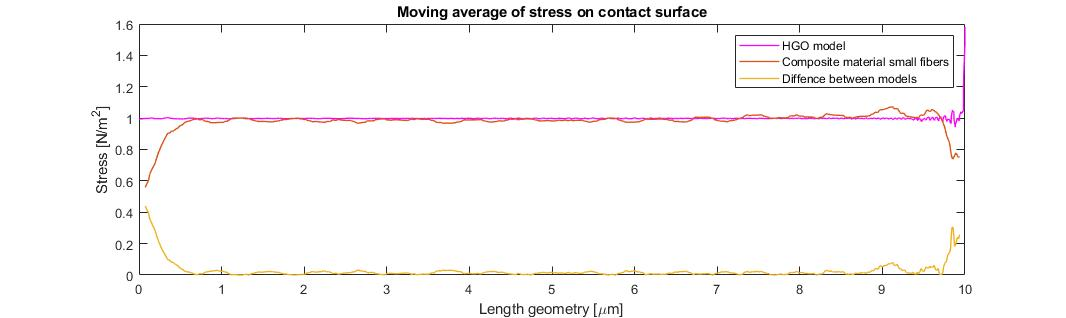
\includegraphics[width=\linewidth, height=3cm, angle=0]{Pictures/validation/validatie_HGO_en_fine_fibers.jpg}
%     \caption{Stress in the HGO model and the fine finer model and the difference between these.}
%     \label{fig:HGO_and_fine_fibers}
% \end{figure}



% de krachtenverdeling wordrt bepaald door de verhouding tussen W1 en W4. dit zijn de isochoric strain energy densities. 

% the isochoric strain energy density relates the strain energy density to the deformation geradient. 

% for normal hyperelastiv materials Comsol computes the second piola kirchhoff stress as 

% \begin{equation}
%     S = 2\frac{\delta W_s}{\delta C}
% \end{equation}

% with W for the strain energy density and C for the right gachy green deformation tensor. 

% for isochoric materials(with a constant volume) a weak constraint is added in the form of $J_{el} = 1$ the auxiliary pressure variable acts as a lagrange multiplier to enforce this constaint. The eqaution for the piola kirchhoff stress is than defined as follows:

% \begin{equation}
%     S =  -p_{w}JC^{-1} + 2\frac{\delta W_{iso}}{\delta C}
% \end{equation}

% $W_{1}$ and $W_{4}$ are both isochoric components. The difference is in the domain they represent. $W_1$ is for the isotropic material properties and $W_4$ is for the anisotropic material properties. 

% Strain for both components is the same for the same location. The ratio between $W_1$ and $W_4$ however is different when the ratio between Cm and k1 is varied. 



% Strain stiffening is iets dat hoort bij de materialen die in de natuur voorkomen, hier nog wel bronnen bij vermelden! hiervoor kun je terugverwijzen naar de vorige onderdelen. De effecten die hier door strain stiffning geintroduceerd worden kunnen dus zeker heel reel zijn


% niet linear gedrag met strain stiffening is gematcht aan het HGO model door Holzapfel et al \cite{holzapfel2000new}
